\documentclass{article}
\usepackage{amsmath, amssymb, graphicx} % For advanced math formatting

\title{Spatial Statistics Exercises Lecture 2}
\author{Tanja Bugajski}
\date{\today}

\begin{document}

\maketitle
\section*{Exercise 1}
Consider a Poisson process $X$, on the unit square, with intensity function $\rho(x,y)=400y$. 
Calculate the mean number of points.\\
Which of the following point patterns could reasonably be a simulation of $X$. 
Which Poisson processes could the others be coming from?
\begin{figure}[h!]
    \centering
    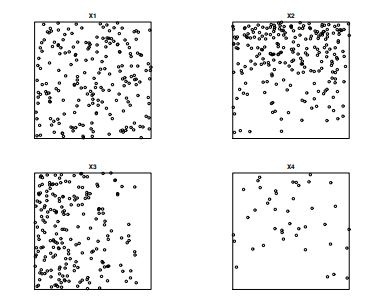
\includegraphics[width=\textwidth]{Ex2.JPG}
    \caption{Examples for Exercises.}
\end{figure}
\subsection*{$(1)$  }
The mean number of points, is found by integrating the intensity function over the region $[0,1]\times [0,1]$:
\[
\mu=\int_{0}^{1}\int_{0}^{1} \rho(x,y)\text{d}x \text{d}y,
\]
Insert:
\[
\mu=\int_{0}^{1}\int_{0}^{1} 400y \text{d}x \text{d}y=
\] 
Integrate:
\[
\mu=\int_{0}^{1}\int_{0}^{1} 400y \text{d}x \text{d}y=\int_{0}^{1}400y \text{d}y=400\int_{0}^{1}y \text{d}y=400\left[1/2y^2\right]_0^1=200.
\] 
Thus, the mean number of points is 200.\\

A reasonable simulation would have a higher concentration of points near the top of the unit square and fewer points near the bottom, reflecting the increasing intensity function $\rho(x,y)=400y$.
Thus, the answer is $x2$.\\

For the other plots:
\begin{itemize}
    \item $x1$ is a uniform Poission process, meaning that the intensity function is constant everywhere i.e.,
    \[ 
    \rho(x,y)=\lambda\ \quad \text{for}\ \lambda> 0.
    \]
    \item $x3$ is concentrated to the left, thus $\rho(x,y)=400(1-x)$.
    \item $x4$ is concentrated around the top, but with fewer points, thus $\rho(x,y)=1/4\cdot 400 y$.
\end{itemize}




\section*{Exercise 2}
An insurance agent is trying to estimate the number of car accidents paid by the insurance company during a given year. Let $t \in [0, 12)$ denote time during the year and assume an inhomogeneous Poisson process of car accidents on this interval with intensity function
\[
\rho(t) = \begin{cases} 
\alpha, & \text{if } t < 3 \text{ or } t \geq 10, \\
\beta, & \text{if } 3 \leq t < 10,
\end{cases}
\]
where $\alpha > \beta$ due to the possibility of slippery roads.

\begin{enumerate}
    \item[(a)] Using this model, find the mean number of car accidents in the Spring ($t \in [2,5)$), if $\alpha = 20$ and $\beta = 10$.
    \item[(b)] What is the probability that no accidents occur in December ($t \in [11, 12)$)?
    \item[(c)] Make an algorithm for simulating this Poisson process (if you like to, you can implement this in R or some other software, but you can also just specify the algorithm on paper).
    \item[(d)] Do you find the model realistic, or do you have suggestions for improving the model?
\end{enumerate}

\subsection*{(a)}
We find the mean number by 
\[
\mathbb{E}[N(B)]=\int_B \rho(t)\text{d}t
\]
Thus,
\[
    \mathbb{E}[N([2,5)])]= \int_{2}^{3}\alpha \text{d}t+\int_{4}^{5}\beta\text{d}t=20\int_{2}^{3}\text{d}t+10\int_{4}^{5}\text{d}t= 20(3-2)+10(5-3)=40
\]
\subsection*{(b)}
For a Poisson process, the probability of zero events in an interval B is given by the void probability formula:
\[
P(N(B=0))=\exp(-\mu(B))=\exp(-\int_B \rho(t)\text{d}t).
\]
Fro Dec. we have $t\in [11,12)$ and $\rho(t)=\alpha=20$:
\[
    \mu([11,12)])=-\int_{11}^{12} 20 \text{d}t=20
\]
Thus;
\[
\exp(-20)\approx 2.06\times10^{-9},
\]
close to zero.
\subsection*{(c)}
Algorithm for simulating this Poisson process:
We simulate an inhomogeneous Poisson process on the interval $[0,12)$ with intensity function  
\[
\rho(t) =
\begin{cases}
\alpha, & t < 3 \text{ or } t \geq 10, \\
\beta, & 3 \leq t < 10.
\end{cases}
\]
where $\alpha > \beta$ due to the possibility of slippery roads.

\textbf{Steps:}
\begin{enumerate}
    \item Set $t = 0$ and initialise an empty list for event times.
    \item Define $\rho_{\max} = \alpha$ as the upper bound for the thinning algorithm.
    \item \textbf{While} $t < 12$:
    \begin{enumerate}
        \item Generate an interarrival time $U \sim \text{Exp}(\rho_{\max})$ and set $t \leftarrow t + U$.
        \item If $t \geq 12$, stop.
        \item Generate a uniform random variable $V \sim U(0,1)$.
        \item Compute the acceptance probability:  
        \[
        p(t) = \frac{\rho(t)}{\rho_{\max}}.
        \]
        \item If $V \leq p(t)$, accept $t$ as an event time.
    \end{enumerate}
    \item Return the list of accepted event times.
\end{enumerate}

\subsection*{(d)}
\subsubsection*{Pros:}
\begin{itemize}
    \item The model captures seasonality, with higher accident rates during the winter months.
    \item It is simple and computationally efficient.
\end{itemize}

\subsubsection*{Cons and Possible Improvements:}

\begin{itemize}
    \item \textbf{No daily variations:} Accidents may follow daily traffic patterns, such as peak hours. A time-dependent function $\rho(t)$ capturing rush hours could improve realism.
    \item \textbf{No spatial effects:} Accidents may be clustered in specific areas, such as highways or intersections. A spatial Poisson process could improve accuracy.
    \item \textbf{No weather dependence:} If real data were available, $\rho(t)$ could be modified based on actual weather conditions, such as snowstorms.
    \item \textbf{Possible model refinement:} A more sophisticated model might define $\rho(t)$ as a smooth function, for example, using a spline or sinusoidal variation, instead of piecewise constants.
\end{itemize}




\end{document}